\section{Castle of Dynamia}
%\begin{figure}[H]
%  \centering
%  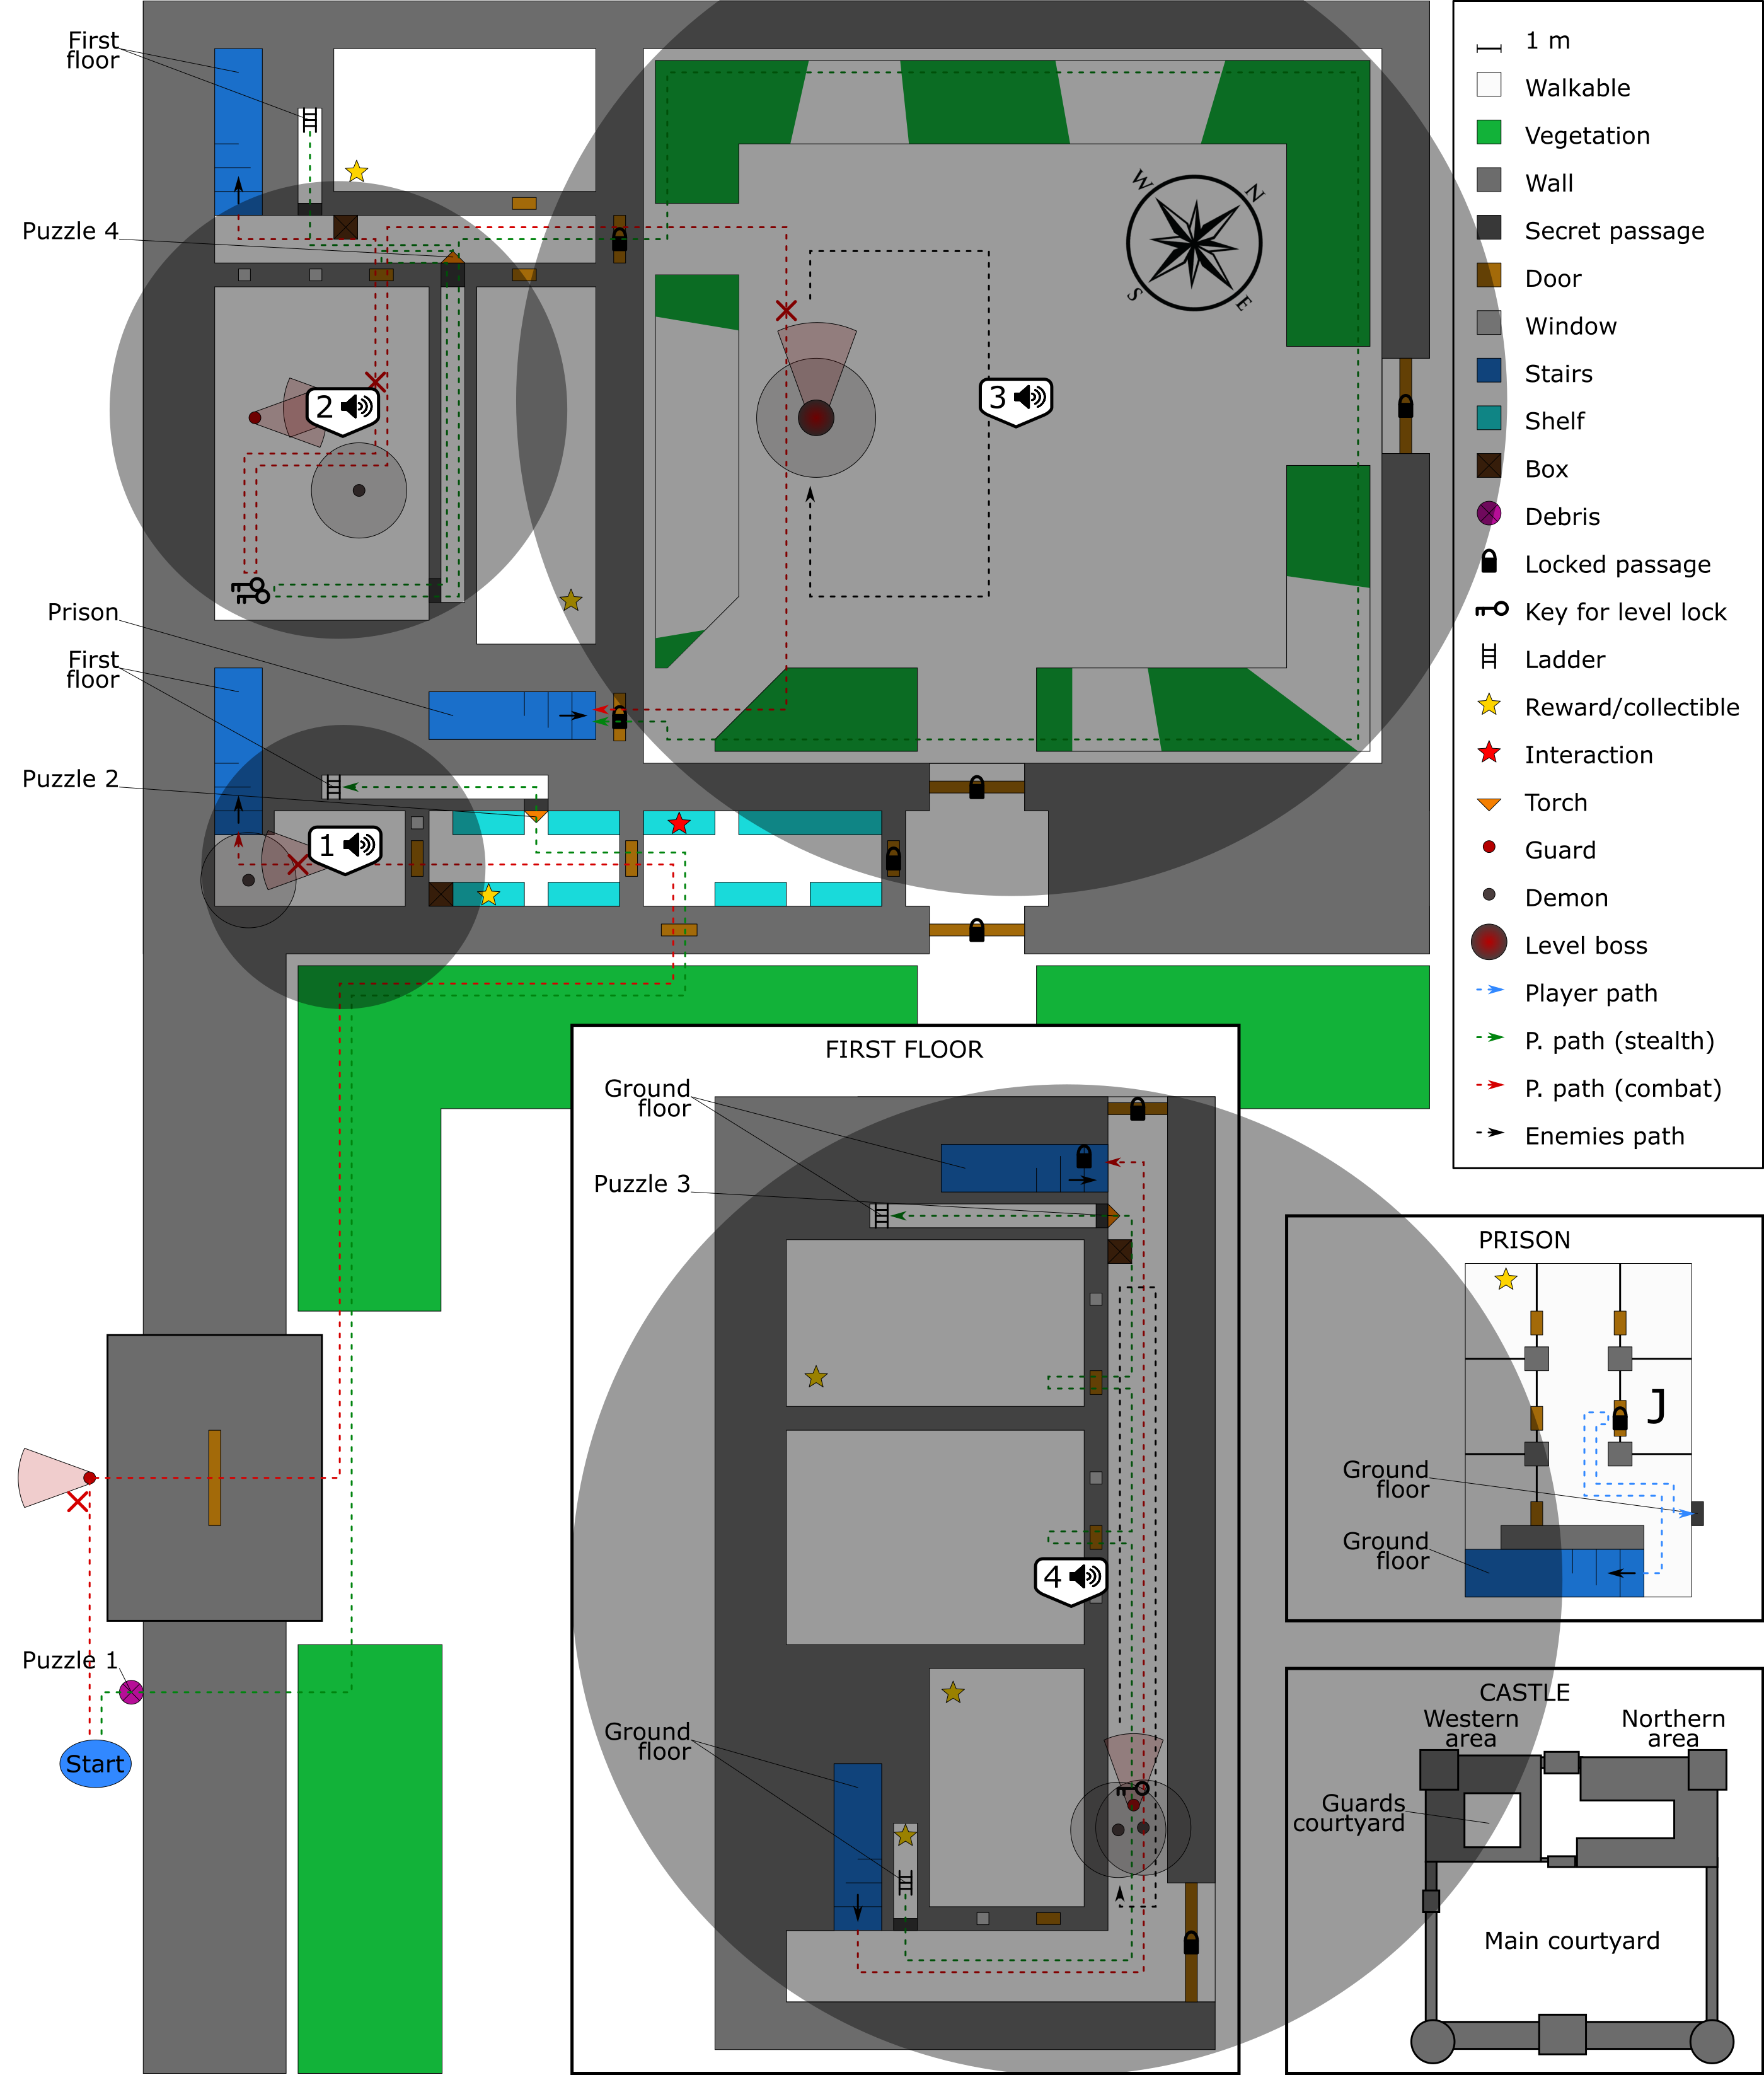
\includegraphics[width=\textwidth]{Images/Maps/castleOfDynamiaAudio}
%  \caption{Audio points for the Castle of Dynamia}
%\end{figure}

In general the castle is pretty quiet.

Inside the castle the floors are made of stone, so the step sound is a little different. In the courtyards the sound is of steps on dry ground. When the player hides in the vegetation, the step sound is muffled and you can hear the rustling of the leafs.

\subsection{Ground floor}
In the main courtyard you can hear some sounds from the city.

In the castle you can hear the voices of the guards and the cry of the demons.

In the guards courtyard you hear the sounds made by the captain.

\subsection{First floor}
In the corridor you can hear the steps of the enemies that are louder as they come closer.

You can hear the sounds made by the captain.

\subsection{Prison}
The prison is very quiet, you can hear only Sophie's steps.
